\documentclass[graphics]{beamer}
\usepackage{xcolor}
\usepackage{graphicx}
\usepackage{verbatim}
\usepackage{wrapfig}
\usepackage{tabularx}
\usepackage{multirow}
\usepackage{amssymb}
\usepackage{pifont}
\usepackage{tikz}
\usepackage{multimedia}

\def\Checkmark{\tikz\fill[scale=0.2](0,.35) -- (.25,0) -- (1,.7) -- (.25,.15) -- cycle;} 

\useoutertheme{shadow}
%\usecolortheme{orchid}
\usecolortheme{seahorse}
\newcommand{\cmark}{\text{\ding{51}}}
%\newcommand*{\GtrSim}{\smallrel\gtrsim}

% math commands
\newcommand{\be}{\begin{eqnarray}}
\newcommand{\ee}{\end{eqnarray}}
\newcommand{\beq}{\begin{equation}}
\newcommand{\eeq}{\end{equation}}
\def\simless{\mathbin{\lower 3pt\hbox
      {$\rlap{\raise 5pt\hbox{$\char'074$}}\mathchar"7218$}}}
\def\simgreat{\mathbin{\lower 3pt\hbox
      {$\rlap{\raise 5pt\hbox{$\char'076$}}\mathchar"7218$}}} %> or of order

% variables

\def\toonscale{0.45}
\def\mboxy#1{\mbox{\small #1}}

\defbeamertemplate*{title page}{customized}[1][]
{
  \usebeamerfont{title}\inserttitle\par
  \usebeamerfont{subtitle}\usebeamercolor[fg]{subtitle}\insertsubtitle\par
  \bigskip
  \usebeamerfont{author}\insertauthor\par
  \usebeamerfont{institute}\insertinstitute\par
  \usebeamerfont{date}\insertdate\par
  \usebeamercolor[fg]{titlegraphic}\inserttitlegraphic
}
\begin{comment}
\AtBeginSection[]{
  \frame{
    \frametitle{Outline}
    \tableofcontents[currentsection]
  }
}
\end{comment}


\title{\textcolor{white}{Plasma Lensing: Pulsars and FRBs}}
%\subtitle{}
\author[U. Pen]{{
\textcolor{green}{\small Ue-Li Pen, CITA+Scintillometry collaboration}
}
\\[8mm] 
}
\date{\textcolor{green}{Feb 3, 2018}}


\begin{document}

\frame{
\vspace{-0.5in}
\begin{center}  
%\includegraphics[width=4.4in]{Figures/IMG-0438-by-Andre-cropped.jpg}
\end{center}
\begin{picture}(320,250)
\put(-35,6){
\includegraphics[width=5.1in]{Figures/IMG-7749-ARO-crop.JPG}
}
\end{picture}
\vspace{-4in}
\\
%image credit: NRAO/AUI/NSF
\\
\vspace{1in}
\titlepage
}

%\section*{Introduction}
\section{Introduction}

\begin{comment}
  \subsection{Outline}

  \frame{
    \frametitle{Outline}
    \tableofcontents
  }
\end{comment}

  \frame{
    \frametitle{Overview}
    \begin{itemize}
      \item cosmic plasma lenses: telescopes and microscopes
      \item Black Widow: PSR B1957+20 disected
      \item two screen lenses: repeater FRB121102, FRB110523, GC
        magnetar, BW, crab,
    \end{itemize}
  }


\frame{
    \frametitle{movie}
\movie[width=8cm,height=4.5cm]{movie}{blackwidow.mp4}

credit: NASA's Goddard Space Flight Center/Cruz deWilde
}

\frame{
    \frametitle{Black Widow}
     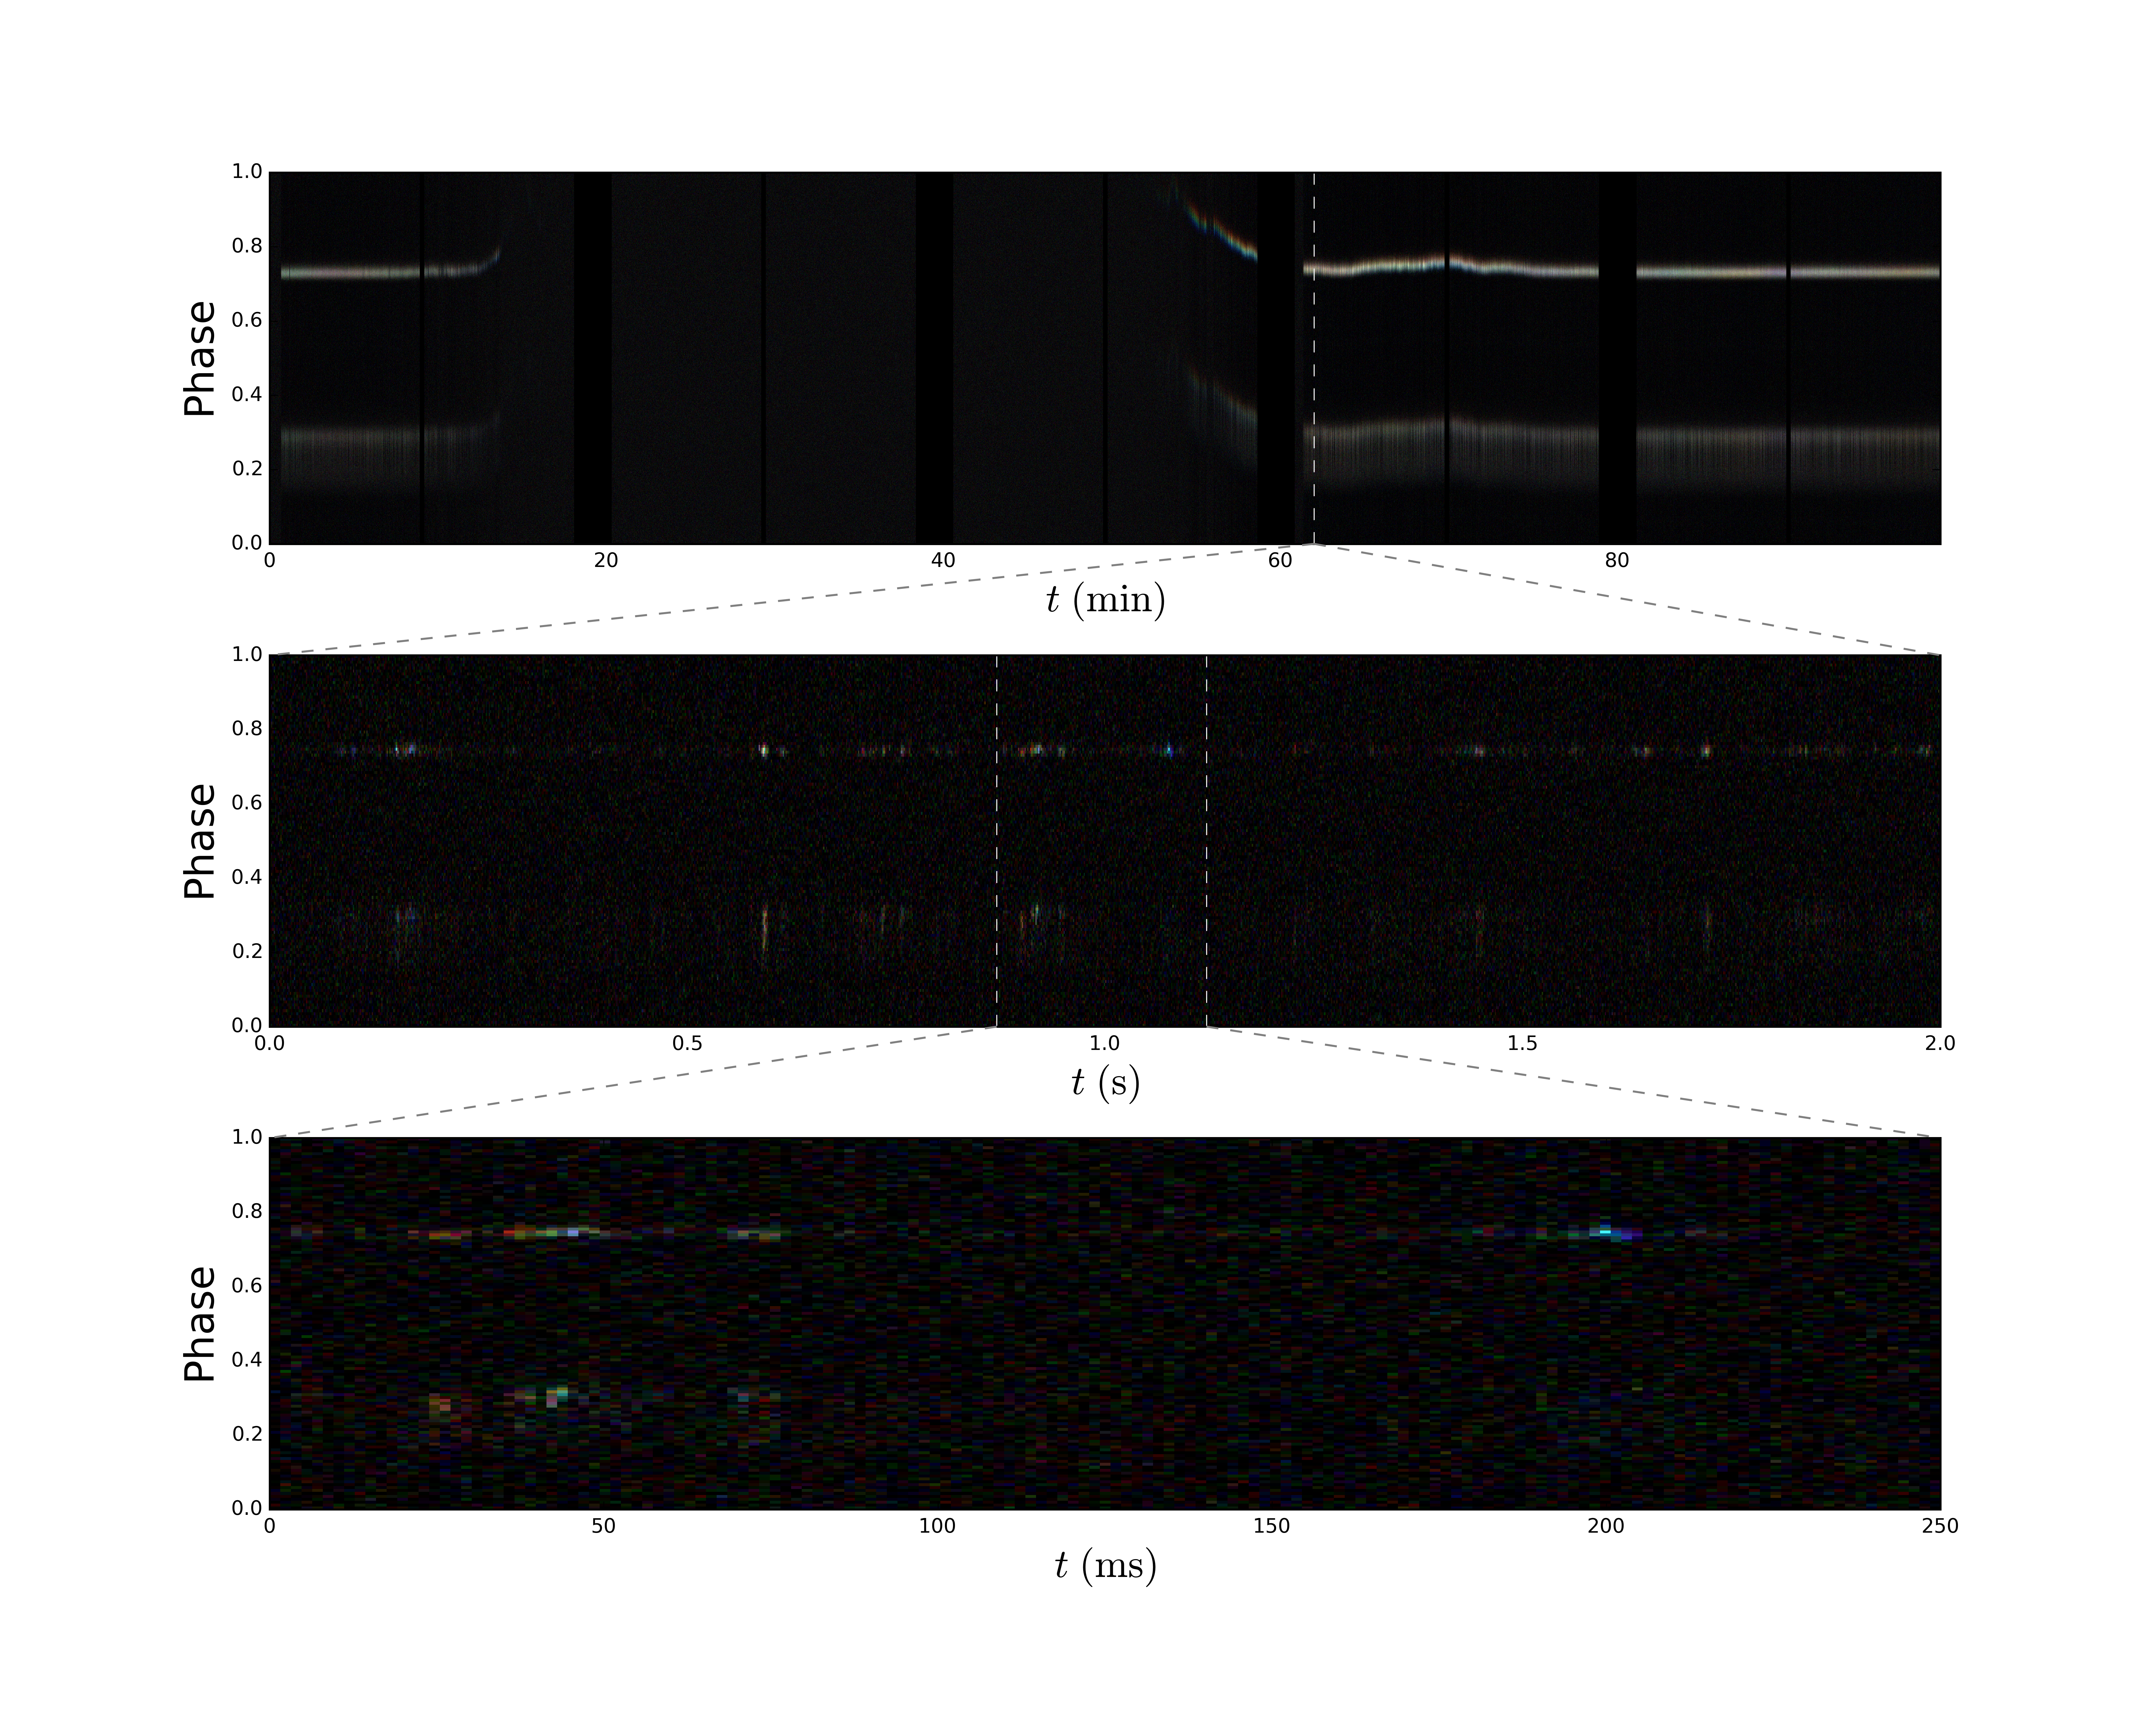
\includegraphics[width=0.8\textwidth]{Figures/LensingPanel-Landscape.png}\\
(Main et al 2018 under review)
}
\frame{
    \frametitle{Zoom}
\includegraphics[width=2.5\textwidth]{Figures/LensingPanel3.png}
}

\frame{
    \frametitle{Black Widow, FRB repeater, Simulation}
\begin{tikzpicture}
    \begin{scope}
    \node
    {\includegraphics[width=0.55\textwidth]{Figures/SpectraPanels.pdf}
};
    \end{scope}
    \begin{scope}[xshift=4cm,yshift=1cm]
      \node
      {
\includegraphics[width=0.45\textwidth]{Figures/Hessels_EDfig1-eps-converted-to.pdf}
};      
    \end{scope}
    \begin{scope}[xshift=5cm,yshift=-2cm]
      \node
      {
\includegraphics[width=0.19\textwidth]{Figures/B1957-SimSpec1-massaged.png}
Main+2018, Michilli+2018, Fang+
};      
    \end{scope}
\end{tikzpicture}

}


\frame{
    \frametitle{Two Screen Lensing}
     \includegraphics[width=1.1\textwidth]{Figures/TwoScreenGeometry.png}

(figure credit: R. Main)
}

  \frame{
    \frametitle{Plasma Lensing}
    \begin{itemize}
    \item observed in pulsars due to companion wind (e.g. PSR B1957+20)
    \item systematic downward drift (seen in FRB121102)  possibly due to screen reflection asymmetry
    \end{itemize}
  }

\section{FRBs}


\frame{
    \frametitle{FRB110523}
     \includegraphics[width=0.4\textwidth]{Figures/nature15769-f1.jpg}
     \includegraphics[width=0.4\textwidth]{Figures/nature15769-sf2.jpg}

Masui et al 2015
}


  \frame{
    \frametitle{Two screen physics}
    \begin{table}
\begin{tabular}{l|rlrl}
object & short & lens & long & lens \\
\hline
FRB110523 &  $\sim 1 \mu$s& galactic & $\sim 1$ms & local
to host \\
FRB121102 & $\sim 10$ns & local to host & $\sim 20 \mu$s & gal plane \\
Black Widow & $\sim 10$ns & companion wind & $\sim 10 \mu$s & galactic
  \\
Crab pulsar& $\sim \mu$s & galactic & $\sim$ ms & nebula \\
GC Magnetar & $\sim $ms (?) & Sgr A* flow & $\sim 1$s & galactic 
\end{tabular}
      \end{table}
  }


  \frame{
    \frametitle{(De-)polarization}
    \begin{itemize}
    \item of all known radio magnetars, 1 in 4(?) has $|RM|>60,000$,
      similar to FRB repeater
    \item magnetar depolarized below 3GHz due to multipath propagation near
      source (Desvignes+ 2018)
    \item if seen from outside galaxy, probably still high RM and
      depolarization, but little scattering.
      \item intriguing parallels: screen due to magnetized accretion flow?
    \item store baseband data!
    \end{itemize}
  }

\section{Summary}

  \frame{
    \frametitle{Conclusion}
    \begin{itemize}
      \item FRB121102: binary plasma lensing?  up to 100x observed for PSRB1957+20
      \item ISM structure: mapping cosmic plasma and magnetic fields
      \item galactic centre magnetar (and maybe crab) important example for
        understanding FRBs
      \item propagation may affect (de-) polarization, high RM
        possible, save baseband data!
      \item future possibilities: CGM, IGM, localization, DM$(z)$ cosmology?

    \end{itemize}
  }

\end{document}
